\section{B-Tree}\label{section:b-tree}

B-Tree is a balanced search tree used for storing large blocks of data. It captures and maintains the sort order of data and supports searching, sequential retrieval, insertion, and deletion in logarithmic time.

Since their invention 50 years ago \cite{bayer-org}, B-Trees have been already considered ubiquitous less than ten years later \cite{10.1145/356770.356776}. They can be found in various forms in databases and file systems, where a performant self-balancing external index for large blocks of data is required.

B-Trees are a specialization of $(a,b)$-Trees, where a B-Tree is either an $(a, 2a)$-tree or $(a, 2a + 1)$-tree depending on the oddness / evenness of $a$. This is also why 2-3-4-trees (which in turn are similar to RB-Trees) are B-Trees with an order of 3.

However, it raises why B-Trees are used for on-disk data, and binary search trees are used for in-memory data. The main reason behind this is the high overhead of data access in block-access storage, where byte access is not well supported. A typical example is disk storage, where a disk is divided into blocks. B-Trees exploit this behavior by having its node be as large as a whole block.

B-Trees are exceptionally useful for secondary disk-based storage, but it still yields significant improvements even when storing data in memory; as with CPU caches and memory line caches, we can treat the memory as a block-access device.

The main benefit of B-Trees is their shallow height even with many keys inserted; thus, the number of disk accesses to traverse the tree is also low.

\begin{figure}[H]
  \centering
  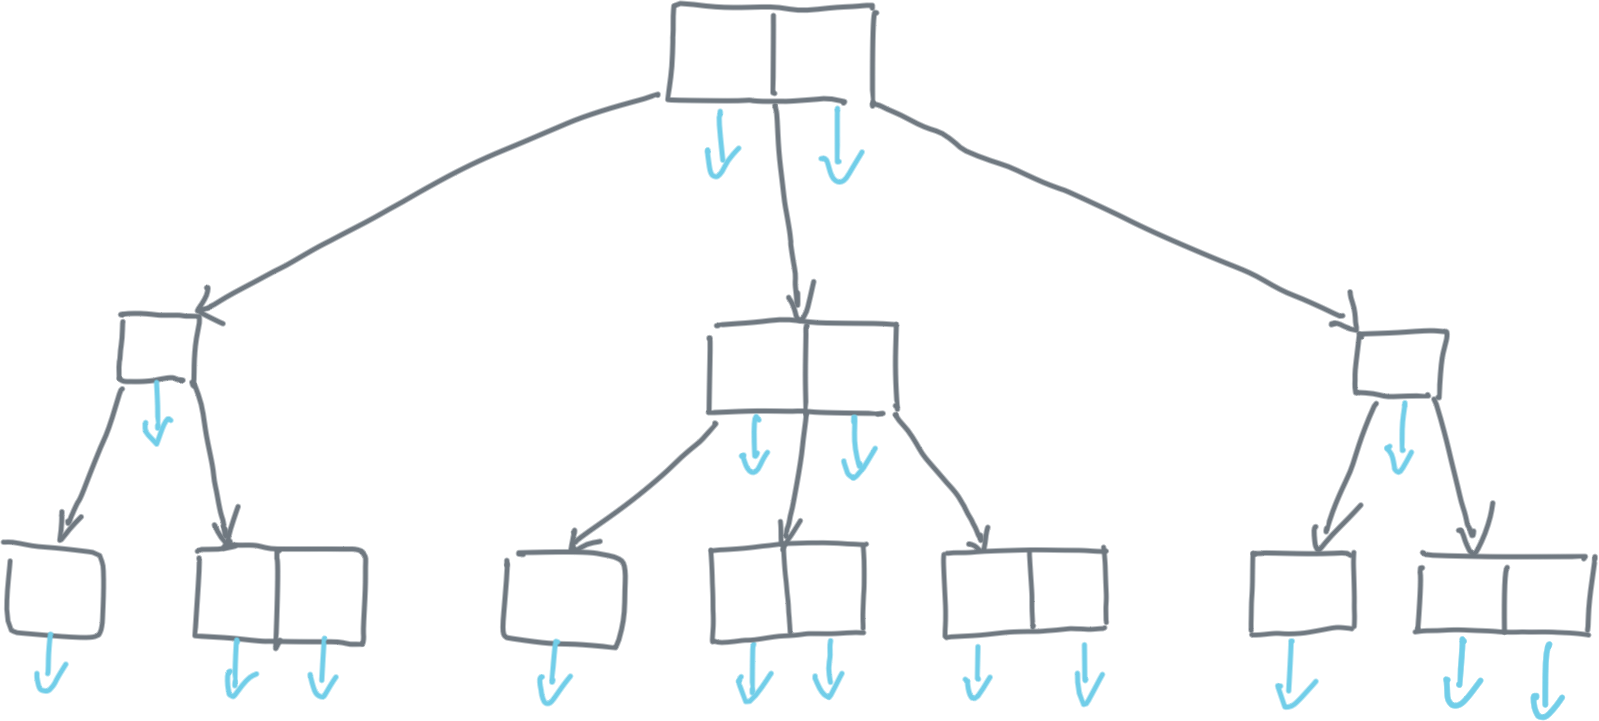
\includegraphics[width=\textwidth]{components/figure/b-tree.png}
  \caption{B-Tree with $Order$ = 3}
  \label{figure:b-tree}
\end{figure}

\begin{definition}\label{def:btree}
  B-Tree of order $m$ is a rooted tree with following properties:
  \begin{enumerate}
    \item Every node $x$ has following attributes:
          \begin{enumerate}
            \item $x.size$, the number of keys in a node,
            \item $x.leaf$, a boolean value indicating whether the node is a leaf or not,
            \item An list of $x.size$ keys $x.key_1, x.key_2, \dots, x.key_{x.size}$ sorted in ascending order ($x.key_1 \le x.key_2 \le \dots \le x.key_{x.size}$),
          \end{enumerate}
    \item Every internal node $x$ has $x.size + 1$ pointers as its children \\($x.child_1, x.child_2, \dots, x.child_{x.size + 1}$),
    \item All leaf nodes appear at the same depth, which is the height of tree $h$,
    \item Nodes have upper and lower bounds, which limit the number of keys and children:
          \begin{enumerate}
            \item Every node other than the root has at least $\floor{\nicefrac{m}{2}}$ children, thus every node other than root has at least $\floor{\nicefrac{m}{2}} - 1$ keys,
            \item The root node has at least two children, except if it is a leaf node,
            \item Every node may contain at most $m$ children, thus may contain at most $m - 1$ keys.
          \end{enumerate}
  \end{enumerate}
\end{definition}

\begin{lemma}
  B-Tree $T$ of order $m$ with $n \ge 1$ keys has height $h = \Theta(\log{n})$.
\end{lemma}

\begin{proof}
  Assume $t = \floor{\nicefrac{m}{2}}$ as the minimum number of children in a node. The root of $T$ has at least one key; all other nodes contain at least $t - 1$ keys.

  Thus, $T$ has at depth $1$ at least $2$ nodes, at depth $2$ at least $2t$ nodes, and so forth, until depth $h$, which has at least $2t^{h-1}$ nodes.

  Define $n_{min}$ as the minimum amount of keys in $T$ of height $h$ as the sum of key count per depth.

  \begin{equation}
    \begin{split}
      n_{min} & = 1 + (t - 1) \cdot (2 + 2t + \dots + 2t^{h-1}) \\
      &= 1 + 2 \cdot (t - 1) \cdot \sum^{h}_{i = 1}{t^{i-1}} = 1 + 2 \cdot (t - 1) \cdot \sum^{h - 1}_{i = 0}{t^{i}} \\
      &= 1 + 2 \cdot (t - 1) \cdot (\frac{t^h - 1}{t - 1}) = 2t^h - 1
    \end{split}
  \end{equation}

  The maximum amount of keys at height $h$ is defined similarily:

  \begin{equation}
    \begin{split}
      n_{max} & = (m - 1) \cdot \sum^{h - 1}_{i = 0}{m^i} \\
      &= (m - 1) \cdot (\frac{m^h - 1}{m - 1}) = m^h - 1
    \end{split}
  \end{equation}

  As $n_{min} \le n \le n_{max}$, taking logarithm will prove the theorem.
\end{proof}

As search, insertion, and deletion on a single node takes $\Theta{(1)}$, time complexity of every operation is $\Theta{(\log{n})}$. The space complexity for B-Tree is $\Theta{(n)}$.

\subsection{Search}

The search algorithm for B-Trees is trivial but crucial, similar to the search algorithm for binary search trees. We compare the keys in every node and decide the subtree to continue the search starting from the root node. The search ends if we find the desired key or if we end up in a leaf node.

\begin{algorithm}
  \caption{B-Tree Search}\label{alg:b-tree-search}
  \SetKwInOut{Input}{Input}
  \SetKwInOut{Output}{Output}
  \DontPrintSemicolon

  \SetKwFunction{Search}{Search}
  \SetKwFunction{UpperBound}{UpperBound}

  \SetKwProg{Fn}{Function}{:}{}
  \Fn{\Search{$node$, $needle$}}{
    $i \gets 0$\;

    \While{$i < node.size$ $\&\&$ $needle > node.key_i$}{
      $i \gets i + 1$\;
    }

    \If{$node.key_i$ = $needle$}{
      \KwRet{$($$node$, $i$$)$}\;
    }

    \If{node.leaf = \textbf{true}}{
      \KwRet{null}\;
    }

    \KwRet \Search{$node.child_i$, $needle$}\;
  }
\end{algorithm}

Line 3--4 in the sample Algorithm \ref{alg:b-tree-search} can be replaced with a binary search or parallelized search in CUDA, which is more suited towards SIMD systems.

\subsection{Insertion}

First, we traverse the tree for the existence of the key. The algorithm will end up in a leaf node if the key is not found. Thus, we need to add the key to the parent of the found node

If a node after insertion has subsequently become full after insertion, a split operation must occur to preserve the invariants of the B-Tree \ref{def:btree}. The node is considered \textit{full} if the node contains exactly $m - 1$ keys. The median key is chosen as the separator, and the node is split into two smaller nodes based on that separator. The separator is inserted into the parent of the split node, which might trigger the split operation again.

When the root node needs to be split, a new node with the separator as its only key and two subtrees as its children, which the definition \ref{def:btree} permits (only internal nodes must contain at least $\floor{\nicefrac{m}{2}}$ keys).

\subsection{Deletion}

Deletion in B-Trees is analogous to insertion. We start by searching the tree for the desired key.

If the key is found on a leaf node, we can trivially delete the key from the node. If the node has subsequently become \textit{underfull} by not containing at least $\ceil{\nicefrac{m}{2}}$ keys, the tree must be rebalanced.

Deleting a key from an internal node is more complicated, as child nodes are bound to keys, and a key deletion will result in the loss of a child. Thus, instead of deleting, we swap the key with a successor (or predecessor) key. The key can then be deleted as it is located in a leaf node after the swap. Similar rebalancing must occur if the node has become underfull.

Rebalancing of node $x$ is performed when $x.size = \floor{\nicefrac{m}{2}} - 1$. Assume, without loss of generality, a sibling node $l$ on the left of $x$ exists, and $i$ is the key, which binds the node $n$ to its parent. If a left sibling does not exist, a right sibling is used instead, and the rebalancing operation is mirrored.

If the sibling node $l$ has at least $\floor{\nicefrac{m}{2}} + 1$ keys, we can perform the borrowing operation; the key $i$ is prepended to the node $x$ and the last key of $l$ detaches from $l$ and replaces the key $i$. Last child of $l$ is also detached and prepended to $x$.

However, if neither the sibling nodes have enough keys, a merge operation occurs. Both the $x$ node and its sibling $l$ are deleted, and a new node is created instead. This new node contains keys and children of both $x$ and $l$, with key $i$ in the middle. Deletion is, thus, propagated upwards. In the event of a root with no keys and a single child, the single child becomes the new root.

Many implementations forgo rebalancing the tree in favor of deleting the key instead of leaving a ghost entry, which can be utilized to alleviate the cost of inserting a new key into a sorted list. Rebalancing the tree can be postponed and executed later.

